\documentclass[tikz,border=9pt]{standalone}
\usepackage{amsmath}
\usetikzlibrary{arrows.meta,calc}
\definecolor{ink}{HTML}{21352F}
\definecolor{teal}{HTML}{087F7B}
\definecolor{blue}{HTML}{4B77A8}
\definecolor{gold}{HTML}{C58B2A}
\definecolor{rose}{HTML}{B65A62}
\definecolor{mercury}{HTML}{8A97A5}
\begin{document}
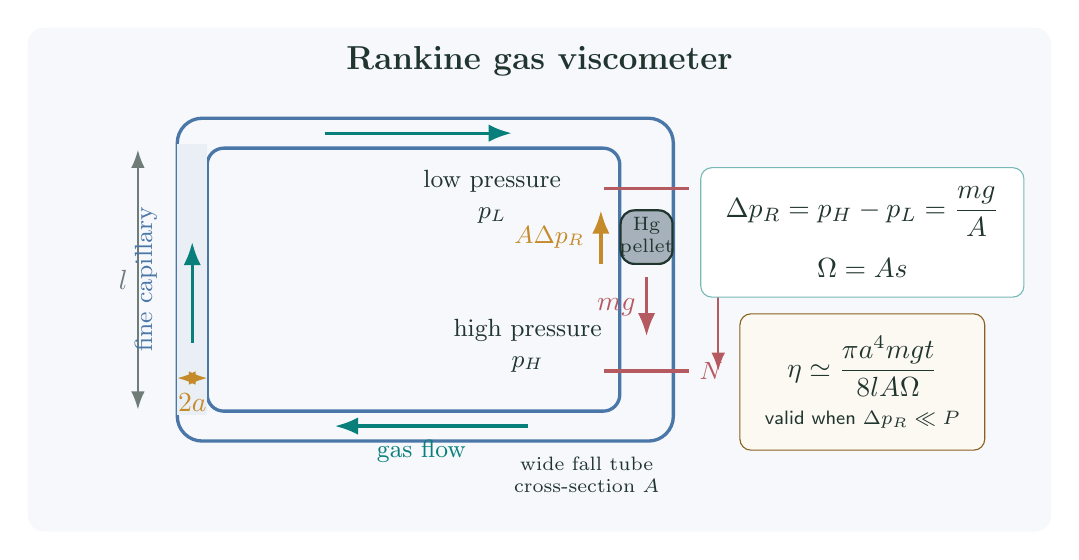
\begin{tikzpicture}[font=\sffamily,text=ink,>=Latex]
  \fill[blue!5,rounded corners=6pt] (-6.5,-3.15) rectangle (6.5,3.25);
  \node[font=\bfseries\large] at (0,2.82) {Rankine gas viscometer};

  \begin{scope}[shift={(-1.45,.05)}]
    % Closed glass loop
    \draw[blue,very thick,rounded corners=9pt]
      (-3.15,2.05)--(3.15,2.05)--(3.15,-2.05)--(-3.15,-2.05)--cycle;
    \draw[blue,very thick,rounded corners=6pt]
      (-2.77,1.67)--(2.47,1.67)--(2.47,-1.67)--(-2.77,-1.67)--cycle;

    % Fine capillary limb
    \fill[blue!12] (-3.15,-1.72) rectangle (-2.77,1.72);
    \draw[<->,gold,thick] (-3.15,-1.25)--(-2.77,-1.25)
      node[midway,below=2pt] {$2a$};
    \draw[<->,ink!65,thick] (-3.65,-1.65)--(-3.65,1.65)
      node[midway,left] {$l$};
    \node[blue,rotate=90,font=\small] at (-3.55,0) {fine capillary};

    % Timing marks
    \draw[rose,very thick] (2.27,1.16)--(3.35,1.16);
    \draw[rose,very thick] (2.27,-1.16)--(3.35,-1.16);
    \node[rose,right,font=\small] at (3.36,1.16) {$M$};
    \node[rose,right,font=\small] at (3.36,-1.16) {$N$};
    \draw[<->,rose,thick] (3.72,-1.16)--(3.72,1.16)
      node[midway,right] {$s$};

    % Mercury pellet
    \fill[mercury!75,draw=ink,thick,rounded corners=5pt]
      (2.48,.20) rectangle (3.14,.88);
    \node[font=\scriptsize,align=center] at (2.81,.54) {Hg\\pellet};
    \draw[->,rose,very thick] (2.81,.03)--(2.81,-.72)
      node[midway,left] {$mg$};
    \draw[->,gold,very thick] (2.23,.20)--(2.23,.88)
      node[midway,left=2pt,font=\small] {$A\Delta p_R$};

    % Pressures and gas-flow direction
    \node[font=\small,align=center] at (1.30,-.84)
      {high pressure\\$p_H$};
    \node[font=\small,align=center] at (.85,1.05)
      {low pressure\\$p_L$};
    \draw[teal,very thick,->] (1.30,-1.86)--(-1.15,-1.86);
    \draw[teal,very thick,->] (-2.96,-.80)--(-2.96,.48);
    \draw[teal,very thick,->] (-1.28,1.86)--(1.10,1.86);
    \node[teal,font=\small] at (-.05,-2.18) {gas flow};
    \node[font=\scriptsize,align=center] at (2.05,-2.48)
      {wide fall tube\\cross-section $A$};
  \end{scope}

  \begin{scope}[shift={(4.10,.10)}]
    \node[draw=teal!55,fill=white,rounded corners=4pt,
      inner xsep=9pt,inner ysep=7pt,align=center] at (0,.55)
      {$\displaystyle \Delta p_R=p_H-p_L=\frac{mg}{A}$\\[7pt]
       $\displaystyle \Omega=As$};
    \node[draw=gold!70!black,fill=gold!6,rounded corners=4pt,
      inner xsep=9pt,inner ysep=8pt,align=center] at (0,-1.35)
      {$\displaystyle \eta\simeq\frac{\pi a^4mgt}{8lA\Omega}$\\[5pt]
       {\scriptsize valid when $\Delta p_R\ll P$}};
  \end{scope}
\end{tikzpicture}
\end{document}
